\chapter{Experimentación}\label{cap:experimentacion}

En este capítulo se muestran los experimentos realizados para evaluar el rendimiento de las Redes Neuronales en la tarea de clasificación de dígitos manuscritos del conjunto de datos MNIST.
Se implementan tanto modelos basados en arquitecturas densas tradicionales como modelos convolucionales, y se comparan sus resultados empleando diversas métricas de evaluación.

\section{Conjunto de datos: MNIST}

El conjunto de datos MNIST (\textit{Modified National Institute of Standards and Technology}) es un benchmark ampliamente utilizado en la literatura de aprendizaje automático \cite{yolo_docs__2024}.
Contiene un total de 70.000 imágenes en escala de grises de dígitos manuscritos (0–9), de tamaño $28 \times 28$ píxeles.

\begin{figure}[h]
	\centering
	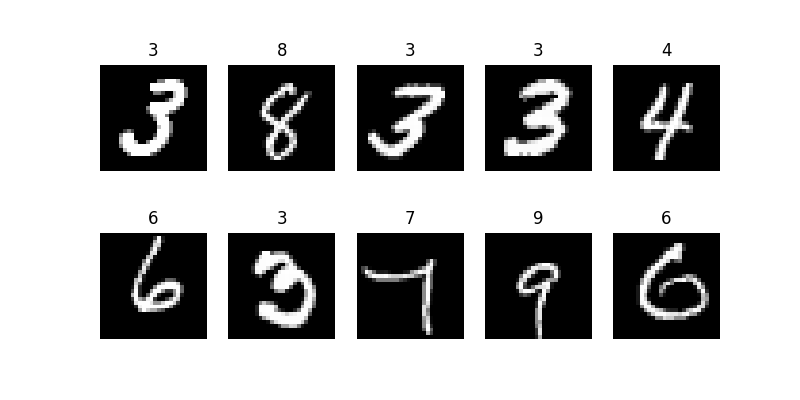
\includegraphics[width=0.6\linewidth]{figures/ejemplos/MNIST_examples.png}
	\caption{Captura de ejemplos aleatorios del conjunto de entrenamiento de MNIST.}
	\label{fig:mnist_examples}
\end{figure}

Este dataset lo segmentaremos en un subconjunto de entrenamiento, del que obtendremos otro subconjunto de validación; y un subconjunto de pruebas. Para ello vamos a utilizar PyTorch \cite{pytorch-web}, una librería de Python para el desarrollo de modelos de aprendizaje profundo optimizada para implementar tensores usando la GPU y la CPU de nuestro ordenador. Por suerte, PyTorch tiene interfaces que nos permiten extraer datasets precargados en sus repositorios de forma muy sencilla.

\begin{lstlisting}[
	language=Python,
	label={code:descargar_mnist},
	caption={Descarga del dataset MNIST.},
	captionpos=b,
	escapeinside={(*@}{@*)}
	]
	from torch.utils.data import DataLoader, random_split
	from torchvision import datasets

	train_dataset = datasets.MNIST(root=datasets_path, transform=ToTensor(), download=True)   (*@\label{line:train_dataset}@*)
	test_dataset = datasets.MNIST(root=datasets_path, train=False, transform=ToTensor(), download=True)   (*@\label{line:test_dataset}@*)
\end{lstlisting}

En \ref{code:descargar_mnist}, la línea \ref{line:train_dataset} descarga y aplica la transformación en tensor mediante \emph{ToTensor()} del conjunto de entrenamiento. Luego, repetimos en la línea \ref{line:test_dataset} para el conjunto de pruebas.

\begin{lstlisting}[
	language=Python,
	label={code:segmentar_dataset_mnist},
	caption={Segmentación del dataset MNIST a conjunto de entrenamiento, validación y pruebas.},
	captionpos=b,
	escapeinside={(*@}{@*)}
	]
	train_size = int(0.8 * len(train_dataset))
	val_size = len(train_dataset) - train_size
	train_subset, val_subset = random_split(train_dataset, [train_size, val_size])   (*@\label{line:split}@*)

	batch_size = 64
	train_dataloader = DataLoader(train_subset, batch_size=batch_size, shuffle=True)   (*@\label{line:train_loader}@*)
	val_dataloader = DataLoader(val_subset, batch_size=batch_size)   (*@\label{line:val_loader}@*)
	test_dataloader = DataLoader(test_dataset, batch_size=batch_size)   (*@\label{line:test_loader}@*)
\end{lstlisting}

A continuación, en \ref{code:segmentar_dataset_mnist}, la línea \ref{line:split} divide el conjunto original de entrenamiento en dos subconjuntos: entrenamiento (80\%) y validación (20\%). Finalmente, en las líneas \ref{line:train_loader}–\ref{line:test_loader} se crean los correspondientes \emph{Dataloaders}, que se encargan de organizar los datos en batches (a los que se le aplica un \emph{shuffle} para el entrenamiento) en cada época, facilitando así el flujo de datos durante las fases de entrenamiento, validación y evaluación del modelo. Dejando nuestro dataset MNIST distribuido como muestra la figura \ref{fig:mnist_distribucion_datasets}.

\begin{figure}[h]
	\centering
	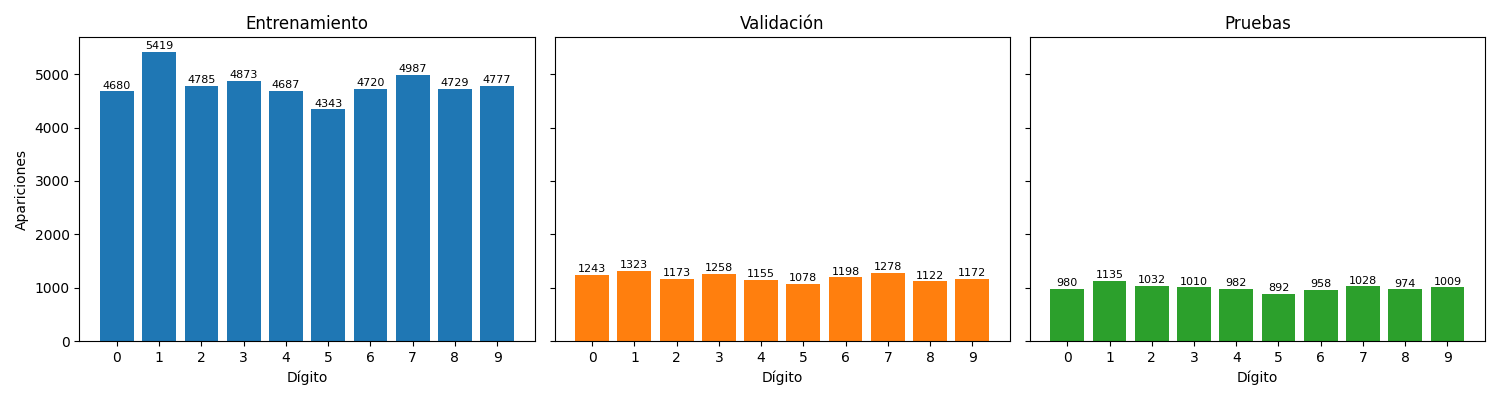
\includegraphics[width=\linewidth]{figures/ejemplos/mnist_distribution_datasets.png}
	\caption{Distribución de muestras de MNIST en los conjuntos de entrenamiento, validación y pruebas}
	\label{fig:mnist_distribucion_datasets}
\end{figure}

\section{Métricas de Evaluación}

Para obtener una visión completa del rendimiento de un modelo, es necesario emplear un conjunto variado de métricas que permitan analizar tanto la calidad global como el comportamiento del modelo en clases individuales, así como su eficiencia computacional y robustez estadística. Estas son las métricas que se utilizarán en el estudio de nuestros modelos \cite{dl_fundamentos__casas_roma_2020}.

\textbf{Exactitud}. La exactitud o tasa de aciertos (TA) relaciona las predicciones correctas con el total de ejemplos:

\begin{equation}
	\text{TA} = \frac{VP + VN}{VP + VN + FP + FN}
	\label{eq:exactitud}
\end{equation}

donde $VP$ son los verdaderos positivos, $VN$ los verdaderos negativos, $FP$ los falsos positivos y $FN$ los falsos negativos. En problemas multiclase se calcula dividiendo el número de predicciones correctas entre el total de muestras. Aunque es una métrica intuitiva, puede ser engañosa en datasets desbalanceados, donde clases mayoritarias dominan el resultado, por ello, hay que tener a mano otras métricas que nos ayuden a compensar.

\textbf{Precisión}. La precisión o valor predictivo positivo (VPP) mide la tasa de ejemplos clasificados como positivos que son realmente positivos:

\begin{equation}
	\text{VPP} = \frac{VP}{VP + FP}
	\label{eq:precision}
\end{equation}

En clasificación multiclase, se calcula de forma independiente para cada clase y luego se obtiene la media. Esto da el mismo peso a todas las clases, lo que evita que clases mayoritarias oculten errores en clases minoritarias.

\textbf{Sensibilidad}. La sensibilidad mide la tasa de verdaderos positivos (TVP) detectados entre todos los ejemplos realmente positivos. Una alta sensibilidad indica que el modelo comete pocos falsos negativos.

\begin{equation}
	\text{TVP} = \frac{VP}{VP + FN}
	\label{eq:sensibilidad}
\end{equation}

\textbf{Pérdida de Entropía Cruzada}. La función de pérdida usada en clasificación multiclase es la entropía cruzada, que mide la discrepancia entre la distribución predicha $\hat{y}$ y la distribución real $y$. Se define como:

\begin{equation}
	\text{PEC} = - \sum_{i=1}^{C} y_i \log(\hat{y}_i)
	\label{eq:perdida_entropia_cruzada}
\end{equation}

donde $C$ es el número de clases, $y_i$ es la etiqueta verdadera codificada en one-hot (1 si la clase es la correcta, 0 en caso contrario) e $\hat{y}_i$ es la probabilidad predicha para la clase $i$.
Un valor de pérdida bajo indica que las probabilidades asignadas por el modelo se aproximan bien a las verdaderas etiquetas \cite{dl_fundamentos__casas_roma_2020, dl__goodfellow_2016}.

\textbf{F1-score}. El cálculo del F1-score consiste en realizar la media armónica entre precisión (\ref{eq:precision}) y la sensibilidad (\ref{eq:sensibilidad}). Este indicador es útil cuando se busca un equilibrio entre falsos positivos y falsos negativos.

\begin{equation}
	F1 = 2 \cdot \frac{\text{VPP} \cdot \text{TVP}}{\text{VPP} + \text{TVP}}
	\label{eq:f1_score}
\end{equation}

\textbf{Tiempo de inferencia por muestra}\label{sec:tiempo_inferencia_muestra}. Con esta métrica somos capaces de estimar el tiempo medio necesario para que el modelo clasifique una única entrada. Se calcula como la relación entre el tiempo total $T$ invertido en clasificar $N$ muestras. Esta métrica toma gran relevancia en aplicaciones en las que la mínima diferencia temporal puede tener repercusiones importantes, por ejemplo, en los vehículos autónomos.

\textbf{ROC-AUC (Área bajo la curva ROC)}\label{sec:roc-auc}. Esta métrica mide área bajo la curva \emph{ROC} (Caracterísica Operativa del Receptor), gráfico que relaciona la sensibilidad o tasa de veraderos positivos (\ref{eq:sensibilidad}) con tasa de falsos positivos $TFP$ (\ref{eq:tasa_falsos_positivos}) para diferentes umbrales de clasificación. Generalmente se utiliza para comparar la robustez entre dos modelos.

\begin{equation}
	TFP = \frac{FP}{FP + VN}
	\label{eq:tasa_falsos_positivos}
\end{equation}

La forma de la curva representa la capacidad de un modelo de clasificación para separar las clases positivas de las negativas. Cada punto de la curva ROC se obtiene variando el umbral de decisión del clasificador. El área bajo esta curva resume en un único valor el rendimiento del modelo en todos los posibles umbrales de decisión.

\begin{figure}[h]
	\centering
	\begin{minipage}{0.49\linewidth}
		\centering
		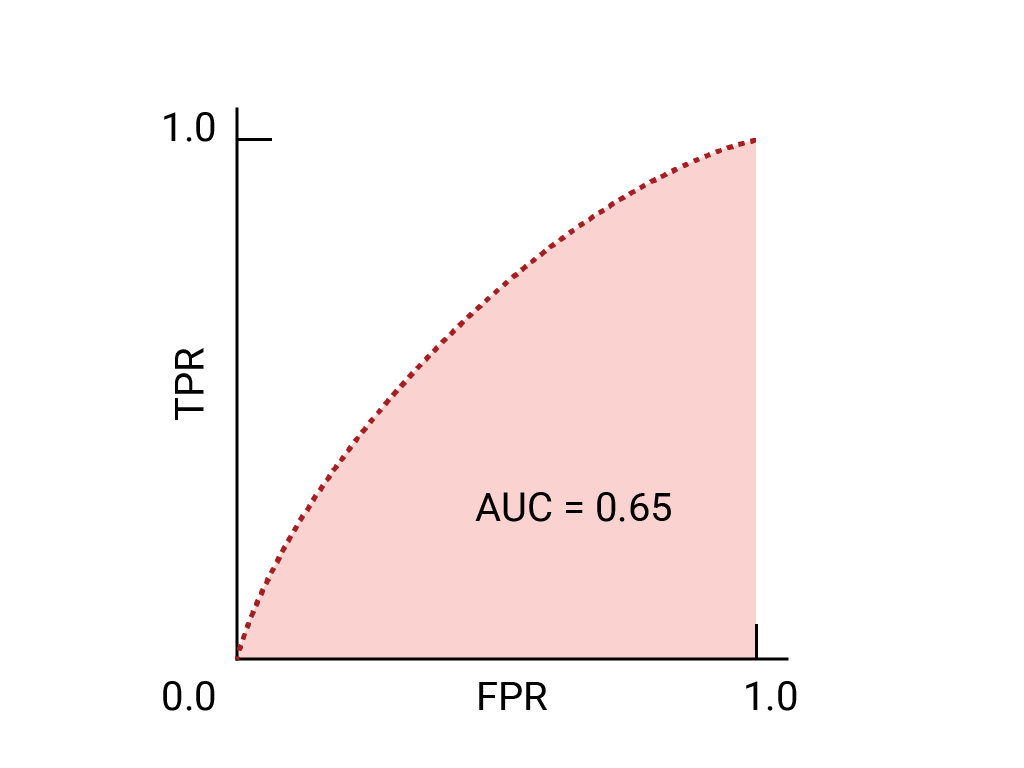
\includegraphics[width=\linewidth]{figures/ejemplos/auc_0-65_google_ejemplo.png}
	\end{minipage}\hfill
	\begin{minipage}{0.49\linewidth}
		\centering
		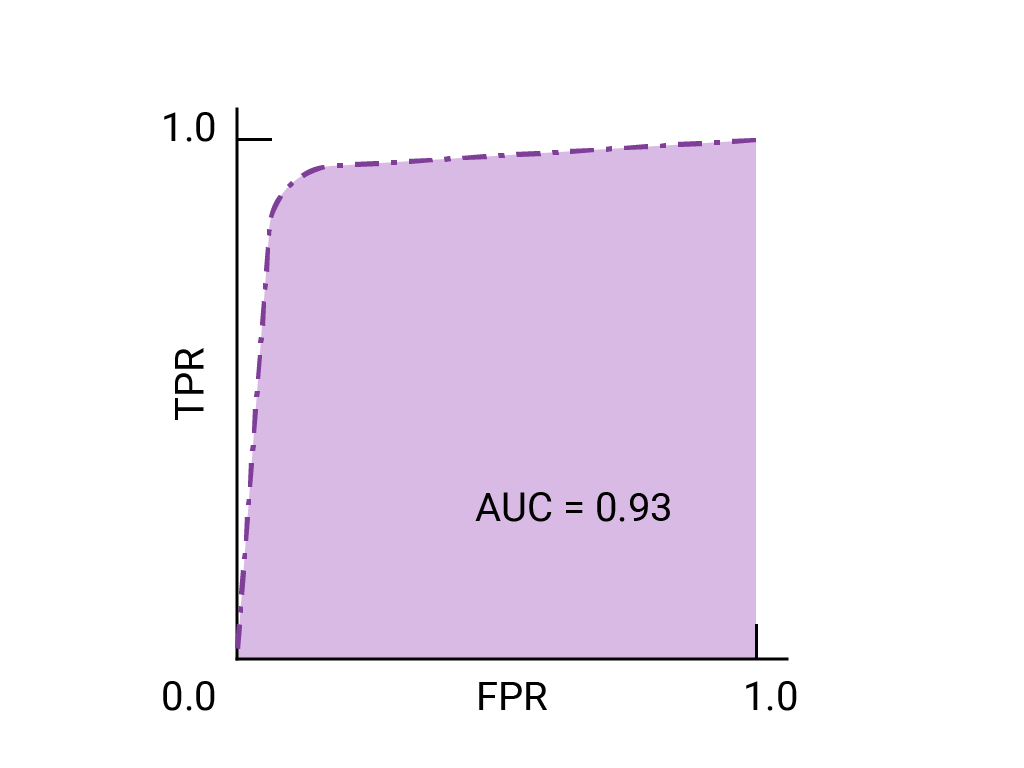
\includegraphics[width=\linewidth]{figures/ejemplos/auc_0-93_google_ejemplo.png}
	\end{minipage}
	\caption{Comparación de áreas bajo la cura de dos modelos de predicción \cite{googledev-rocauc}.}
	\label{fig:auc_65_google}
\end{figure}

Cuando en nuestro dataset existan múltiples clases, se calcula el AUC para cada clase frente al resto, lo que se conoce como \textit{one-vs-rest}, y posteriormente se promedian los valores. Este enfoque permite evaluar de forma equilibrada el desempeño en todas las clases, sin que las más frecuentes dominen la métrica \cite{googledev-rocauc}.

Tomando como ejemplo la figura \ref{fig:auc_65_google}, un valor de AUC que tienda a $1$ indica una buena separación entre clases, lo que significa que el modelo es capaz de asignar puntuaciones más altas a los ejemplos positivos que a los negativos de forma consistente. En cambio, un valor en torno a 0.5 corresponde a un clasificador aleatorio, mientras que valores inferiores a 0.5 denotan un rendimiento peor que el azar, lo que puede indicar un problema en el entrenamiento o en la interpretación de las salidas del modelo \cite{dl_python__chollet_2021}.

\textbf{Matriz de confusión}. Este gráfico resume el rendimiento del clasificador mostrando cómo se distribuyen las predicciones entre las clases. Cada fila representa las instancias reales y cada columna las predicciones. También se pueden normalizar las predicciones dividiendo cada fila por el total de ejemplos de la clase, de modo que cada valor representa un porcentaje. Esto permite identificar qué clases confunde el modelo con mayor frecuencia.

\subsection*{Prueba de McNemar}

{\color{red} AÑADIR TABLA DE MCNEMAR}

La \textbf{prueba de McNemar} es un test estadístico no paramétrico que permite comparar dos clasificadores sobre el mismo conjunto de test.
Se basa en una tabla con los conteos de aciertos y errores de ambos modelos, y se define como:

\begin{equation}
	\chi^2 = \frac{(|b - c| - 1)^2}{b + c}
	\label{eq:mcnemar}
\end{equation}

donde $b$ es el número de muestras mal clasificadas por el modelo A pero correctas en el B, y $c$ el número de muestras correctas en el A pero mal clasificadas en el B.
Un valor de $\chi^2$ mayor que el umbral crítico (dependiendo de $\alpha$) indica que las diferencias entre los modelos son estadísticamente significativas.

\subsection*{Top K Confusiones}

El análisis de las \textbf{top-k confusiones} permite identificar las clases que generan más confusión en el modelo.
Para cada clase verdadera se calcula la tasa de error:

\begin{equation}
	\text{Tasa de Error}_i = \frac{\text{Número de errores de la clase } i}{\text{Total de ejemplos de la clase } i}
	\label{eq:topk}
\end{equation}

y se listan las $k$ clases predichas erróneamente un mayor número de veces.
Este análisis ayuda a entender qué dígitos son más difíciles de distinguir y proporciona información útil para mejorar el modelo.


\section{Implementando una Red Neuronal para Clasificar Números}

Como punto de partida se implementó una red neuronal densa (\textit{Fully Connected Network}) denominada \texttt{SimpleNN}.
Este modelo sirve como \textbf{baseline} al no incorporar capas convolucionales, limitándose a capas densamente conectadas.

La arquitectura está formada por:

\begin{itemize}
	\item \textbf{Capa de entrada:} las imágenes de tamaño $28 \times 28$ píxeles se aplanan en un vector de $784$ componentes.
	\item \textbf{Capa oculta 1:} 512 neuronas, activación ReLU.
	\item \textbf{Capa oculta 2:} 512 neuronas, activación ReLU.
	\item \textbf{Capa de salida:} 10 neuronas, que corresponden a las 10 clases de dígitos, sin activación explícita (los logits se normalizan posteriormente mediante softmax en la función de pérdida).
\end{itemize}

El modelo se entrena con la función de pérdida \textbf{entropía cruzada} y el optimizador \textbf{Adam}.
Pese a su simplicidad, este enfoque permite establecer un punto de comparación frente a arquitecturas convolucionales más complejas.

\section{Implementando una Red Convolucional para Clasificar Números}

Para mejorar la extracción de características espaciales se implementó la red \texttt{SimpleCNN}, una \textbf{Convolutional Neural Network} diseñada específicamente para imágenes en escala de grises de MNIST.

La arquitectura consta de:

\begin{itemize}
	\item \textbf{Capa convolucional 1:} 32 filtros $3 \times 3$, activación ReLU, seguida de max pooling ($2 \times 2$).
	\item \textbf{Capa convolucional 2:} 64 filtros $3 \times 3$, activación ReLU.
	Esta capa almacena internamente sus activaciones y gradientes para técnicas de visualización como Grad-CAM.
	\item \textbf{Max pooling:} ventana de $2 \times 2$ tras la segunda convolución.
	\item \textbf{Capa densa 1:} 120 neuronas, activación ReLU.
	\item \textbf{Capa densa 2:} 84 neuronas, activación ReLU.
	\item \textbf{Capa de salida:} 10 neuronas, correspondientes a las clases de dígitos.
\end{itemize}

La inclusión de capas convolucionales y de pooling permite detectar patrones locales (bordes, texturas, formas simples) y reducir la dimensionalidad manteniendo la información relevante.
Las capas densas finales combinan estas características extraídas para producir la clasificación.
Además, el diseño de \texttt{SimpleCNN} incluye métodos para recuperar activaciones y gradientes de la última capa convolucional, esencial para técnicas de interpretabilidad como Grad-CAM.


\section{Discusión}
